\documentclass{article}

\usepackage{listings} % for including MATLAB code
\usepackage{graphicx} % for including images
\usepackage{amsmath}

\title{80846 - Report - 5th}
\author{GU JUN, 6132230056-4}
\date{\today}

\begin{document}

\maketitle


\section{\centering \Large iterative learning controller}

\subsection*{Problem Statement}

According to the class, we are required to complete the \\
1. learning law block \\
2. iterative learning model based on transport delay block \\


% model of the system
\subsection{Simulink Model}
See the Figure \ref{fig:model_ilc} below. Besides transport delay blocks, I also used the subsystem block and a clock block to restart $q$ every trail. The length of the trail is $1$ second.
\begin{figure}[ht]
    \centering
    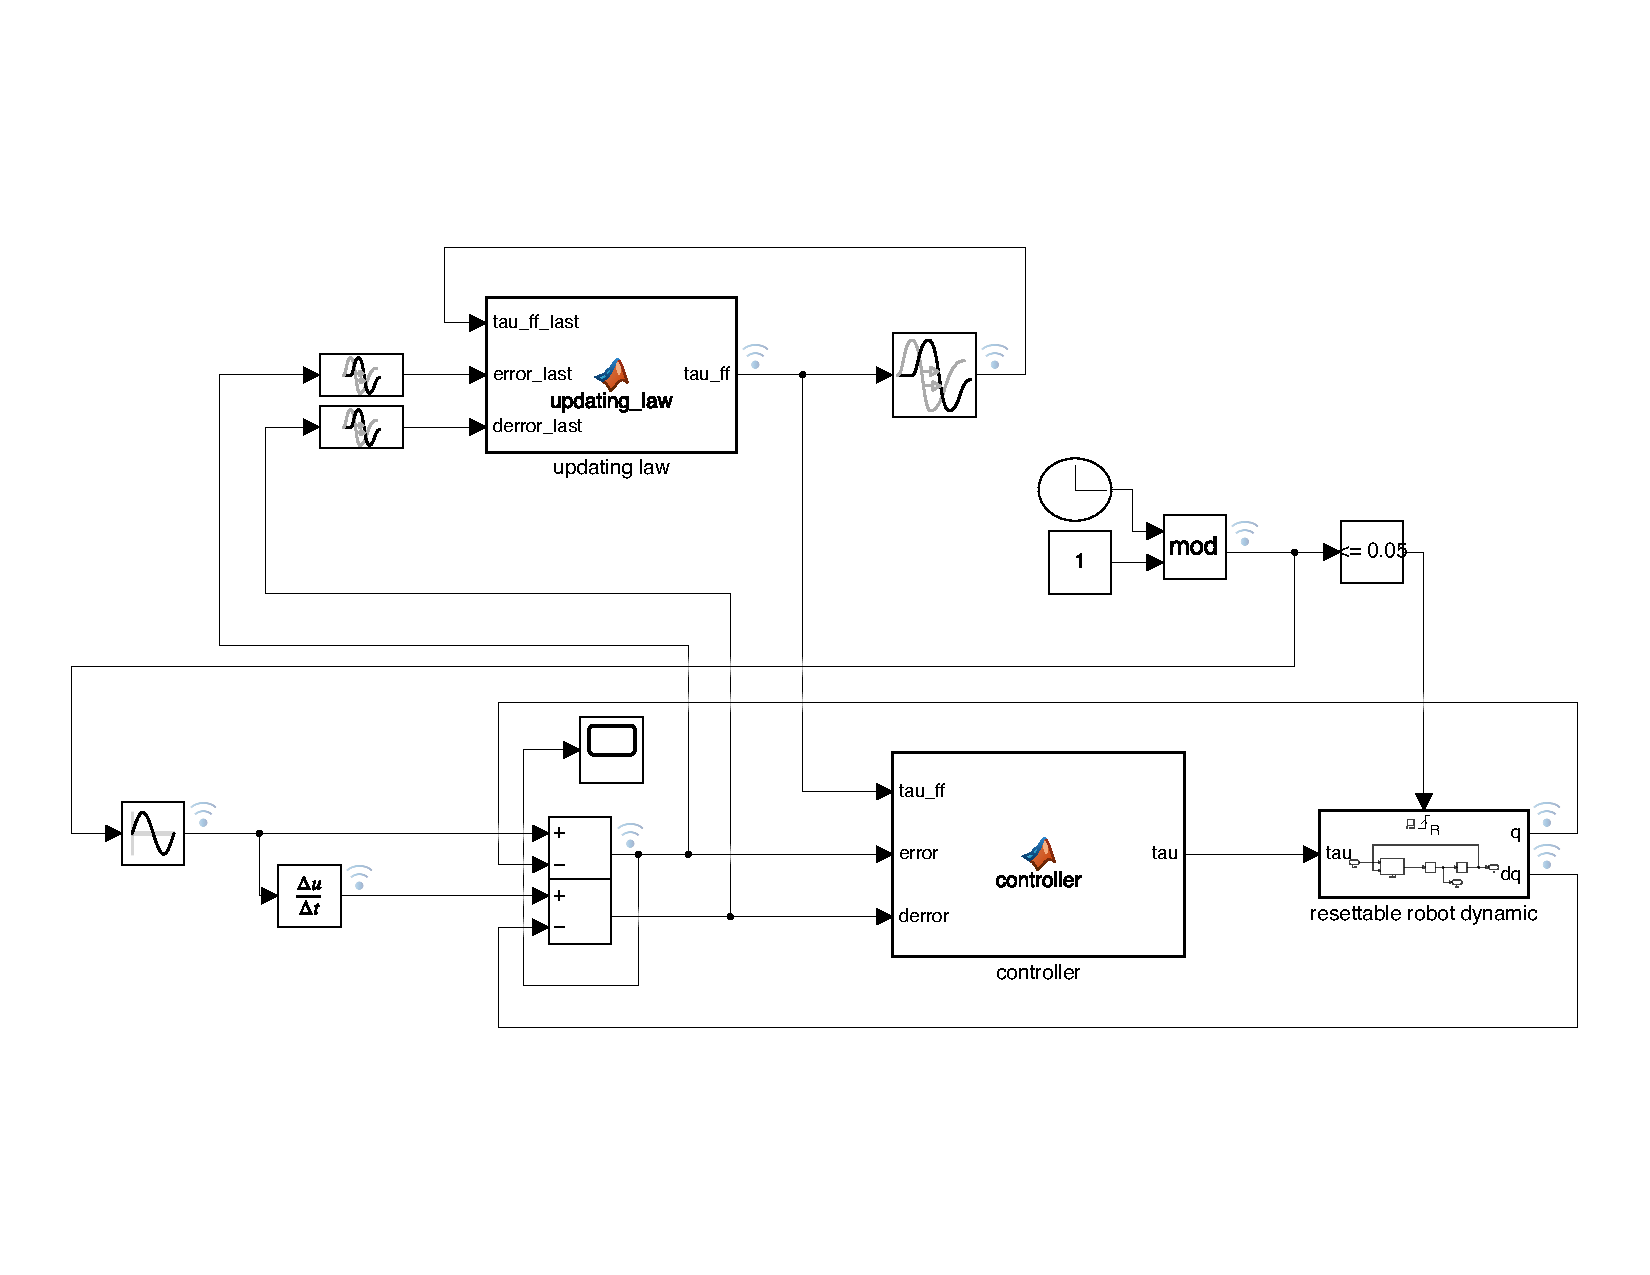
\includegraphics[width=0.9\textwidth]{report/figures/model_ilc.pdf}
    \caption{Simulink Model of the iterative learning controller}
    \label{fig:model_ilc}
\end{figure}

% formulas and source codes
\subsection{Formulas and Source Codes}
This part includes the formulas and source codes for the learning law block
\subsubsection*{learning law}
The feed-forward input is updated by using the control error of the last trial.

$$
\tau_{ff2}(t) = \tau_{ff1}(t) + \alpha(\beta(q_d(t)-q_1(t))+\dot{q}_d(t)-\dot{q}_1(t))
$$
    

The source code is shown below:
\begin{lstlisting}[language=Matlab, basicstyle=\small\ttfamily]

function tau_ff = updating_law(tau_ff_last, error_last, derror_last)

alpha = 0.5;

beta = 20;

tau_ff = tau_ff_last + alpha * (beta * error_last + derror_last);

end

\end{lstlisting}


\subsection{Simulation Results}

As a result, I got the following Figure \ref{fig:result_task_space_plot}, where the desired trajectory is $cos$ wave, and its frequency is $2 \pi$. Because the robot dynamic always restarts in every trail, the error always starts from $1$.
\\
\begin{figure}[ht]
    \centering
    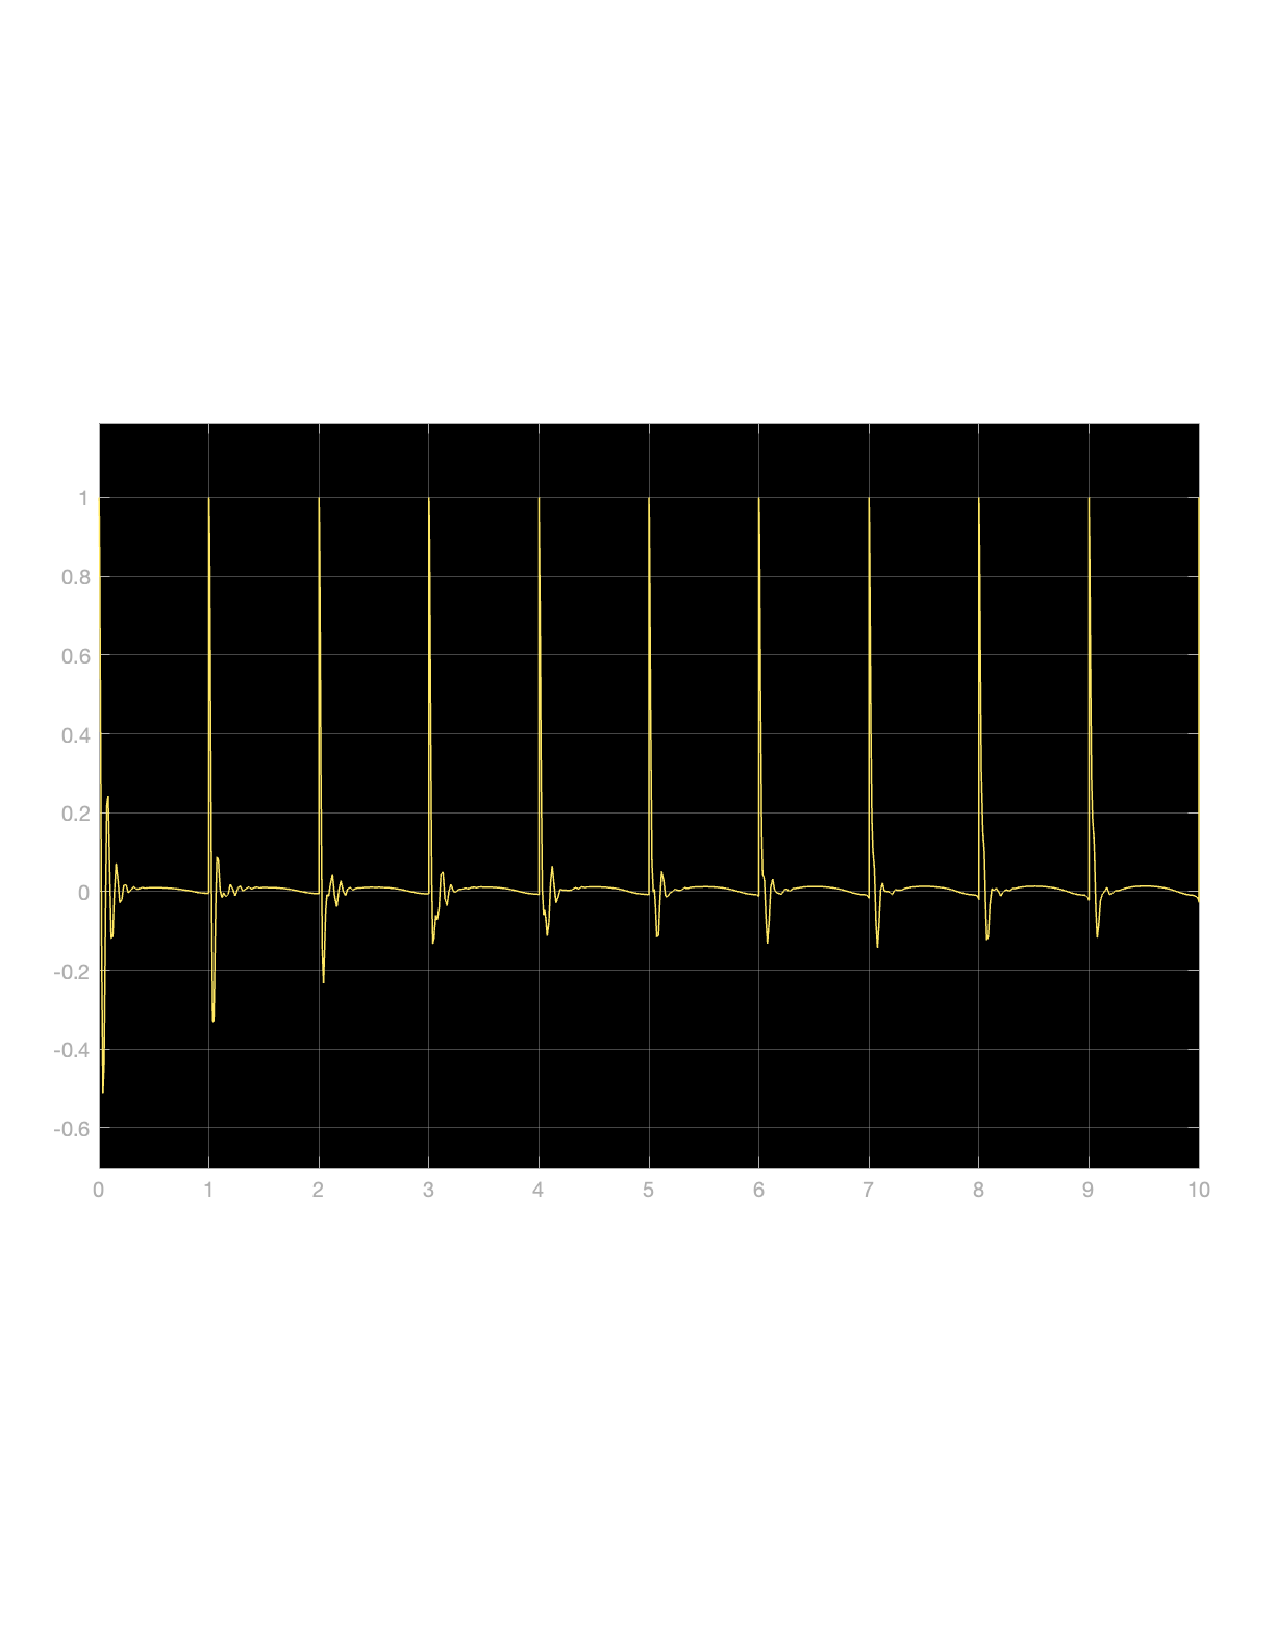
\includegraphics[width=0.8\textwidth]{report/figures/result_ilc.pdf}
    \caption{as you can see, the error is decreasing every trail.}
    \label{fig:result_ilc}
\end{figure}





\newpage

\section{\centering \Large two-joints case} 

\subsection*{Problem Statement}

For the two-joints case, we only need to change the robot dynamic to a two-joints version, we already have done this before, so we can just copy it from the report before.

\subsection{Simulation Results}

There I got this result

\ref{fig:result_ilc_muilt_joints}. \\
\begin{figure}[ht]
    \centering
    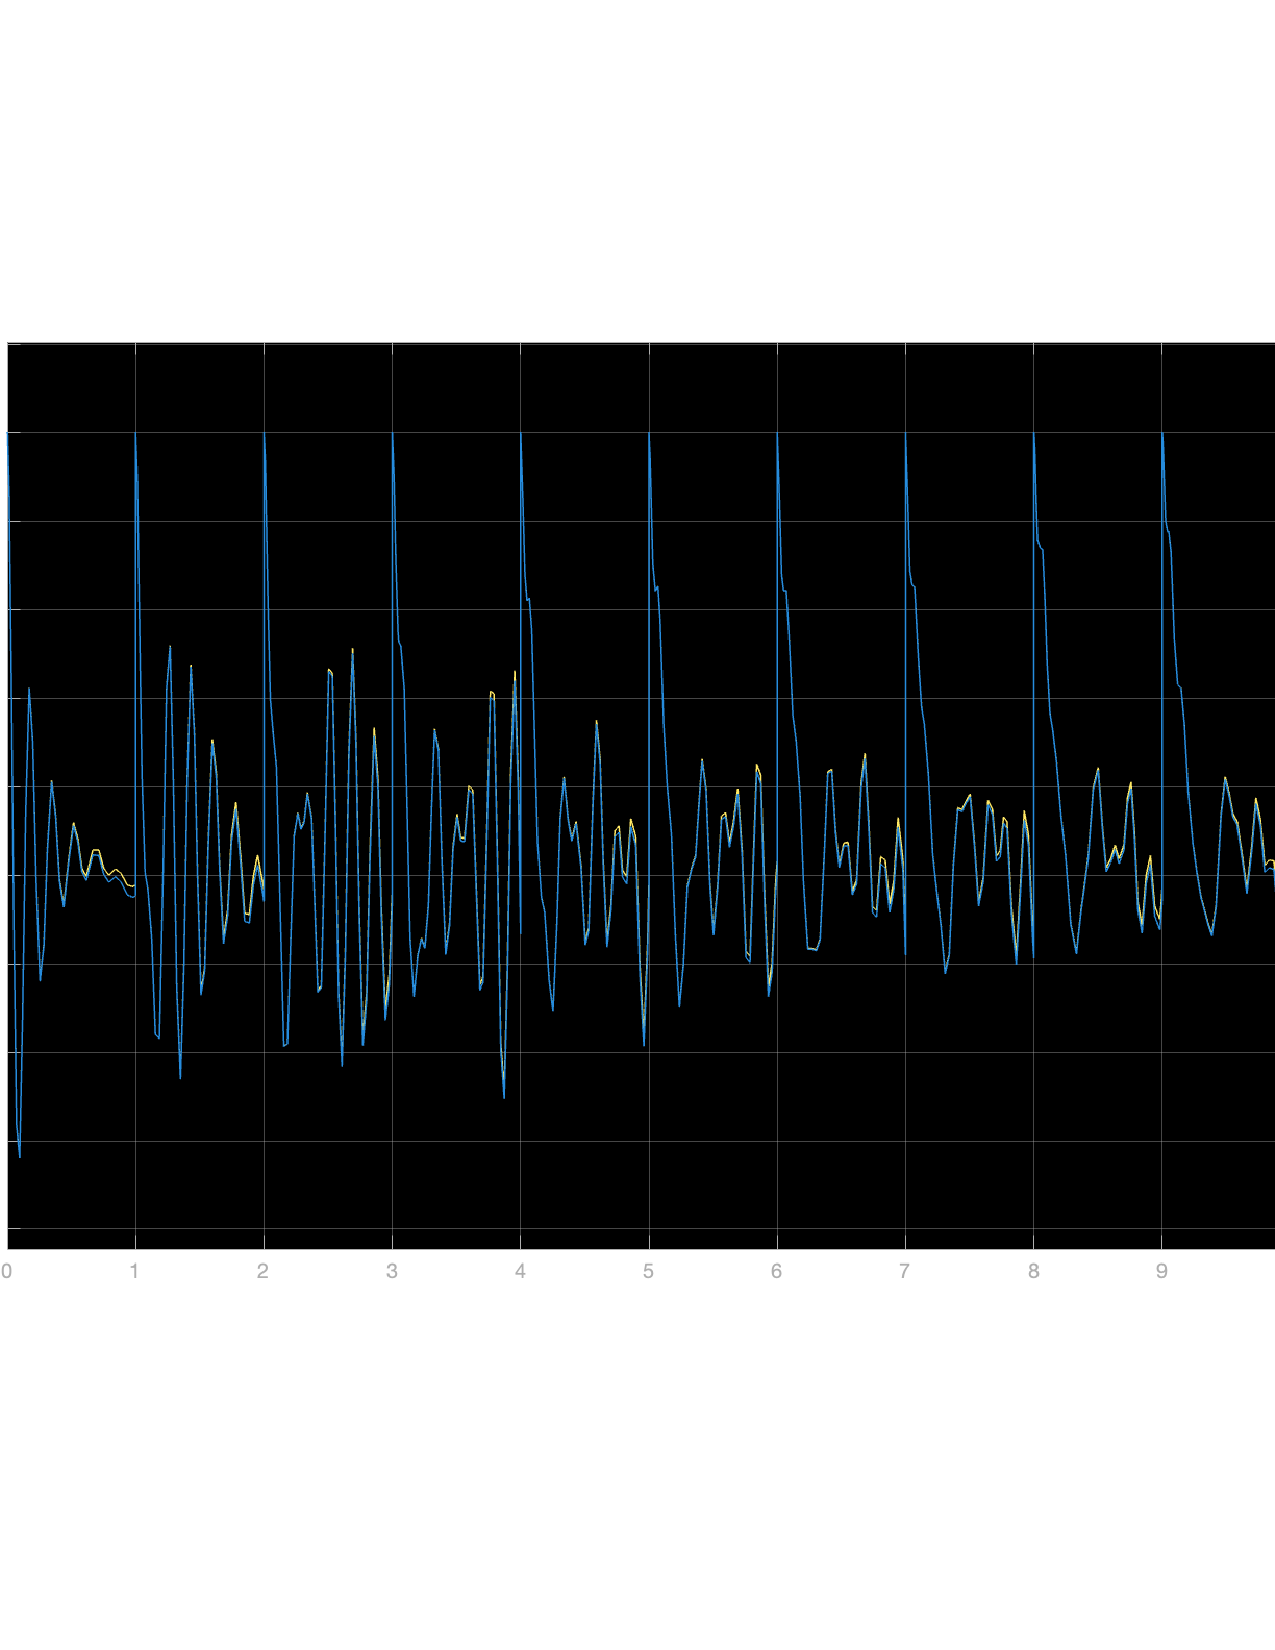
\includegraphics[width=0.8\textwidth]{report/figures/result_ilc_muilt_joints.pdf}
    \caption{The result is not as good as the one-joint case.}
    \label{fig:result_ilc_muilt_joints}
\end{figure}



\newpage

\section{Explanation}



\subsection{iterative learning controller}
Writing the learning block is easy to do, but how to store and read the data from the last trial is harder. Besides the transport delay block, I also used a clock block and re-settable subsystem block to reset the robot dynamic.\\

As you can see, the errors decreased in every trial.
\subsection{two-joints case}
For iterative learning control, it is almost the same as the one-joint case.\\

However, the result is not good as you can see, maybe it is because parameters are not good enough.\\


\end{document}